\documentclass[../TST.tex]{subfiles}
\begin{document}

\begin{pproblem}
Find the equivalent resistance of the circuit on Figure \ref{fig1}. Each segment represents a resistance $R$. Draw the equivalent circuits that you have used to reach the answer.

\begin{figure}[h]
\centering
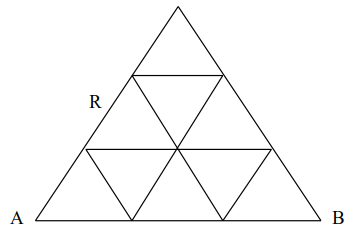
\includegraphics[width=0.4\textwidth]{fig/2009_s5.png}
\caption{}
\label{fig1}
\end{figure}

\end{pproblem}

\ifprob \else
\begin{solution} Similarly to how we set $c=1$ in relativity, let's set $R=1$ and restore the $R$ at the end. First we apply a Y-$\Delta$ transformation on all triangles that point up. We are left with a simpler circuit:
\begin{center}
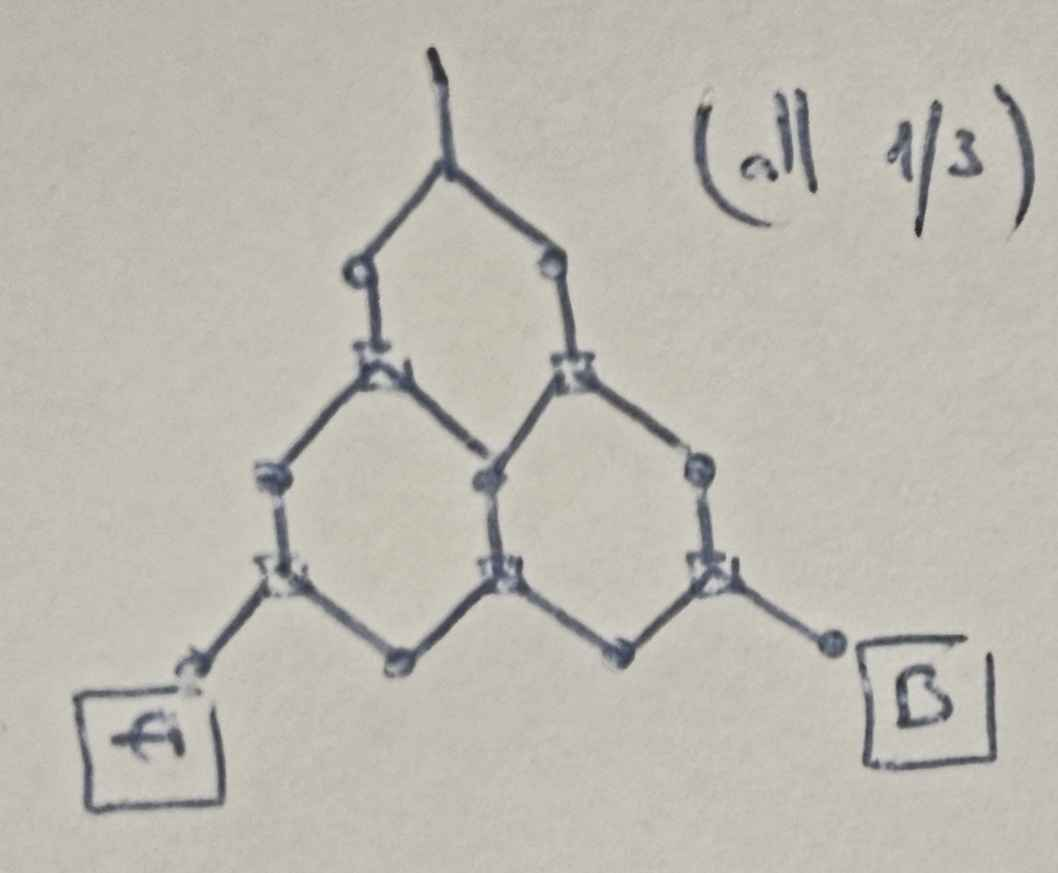
\includegraphics[width=0.3\textwidth]{fig/a2009_s51.jpg}
\end{center}


The resistance at the top doesn't lead anywhere, so we can take it out. After that we can simplify the series connections. Now examine points $E$ and $O$. If the potential at $A$ is $\varphi$ and the potential at $B$ is zero, the potentials at both $E$ and $O$ have to be $\varphi/2$. This is because they lie on a symmetry axis that divides the circuit between $A$ and $B$ into two identical parts. More rigorously, think about how the currents along the path $ACDE$ are the same as those along the path $EFGB$. The resistances are also the same, so the voltage drop between $A$ and $E$ should be equal to that between $E$ and $B$. The total voltage across the circuit is $\varphi$, so each voltage drop is $\varphi/2$.
\begin{center}
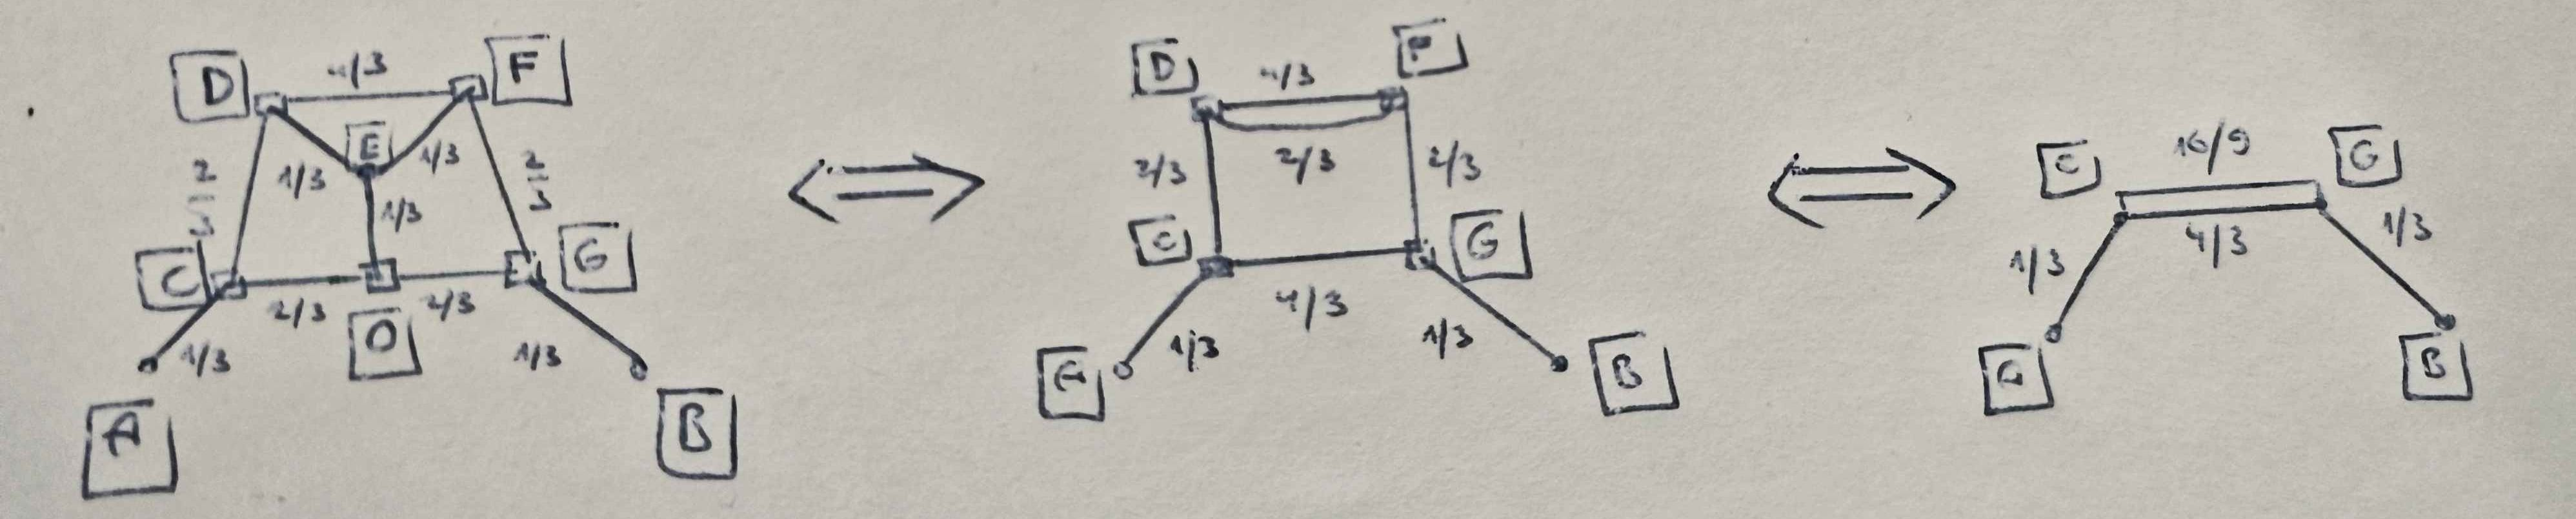
\includegraphics[width=0.95\textwidth]{fig/a2009_s52.jpg}
\end{center}
The potentials at $A$ and $B$ are equal, meaning that no current can flow between them through the resistance $EO$. As a result, removing $EO$ from the circuit then wouldn't change anything. Following that, we will only have to deal with series and parallel connections. The equivalent resistance turns out to be $\frac{10}{7}$, or, after we put the $R$ back, \fbox{$\frac{10}{7}R$.}



\end{solution}
\fi
\end{document}
